\documentclass[a4paper,11pt]{article}

\usepackage[utf8]{inputenc}

\usepackage{graphicx}
\usepackage{caption}
\usepackage{subcaption}

\usepackage{pgfplots}
\usepackage{float}
\usepackage{hyperref}
\usepackage{soul}
\hypersetup{
    colorlinks=true, % Enable colored links
    linkcolor=black, % Color for internal links
    urlcolor=black,  % Color for external links
    citecolor=black, % Color for citation links
    pdfborder={0 0 0}, % Remove border around links
}
\newcommand{\underlinehref}[2]{%
    \href{#1}{\ul{#2}}%
}
\pgfplotsset{compat=1.18}


\usepackage{minted}

\begin{document}

    \title{
        \textbf{Sorting Arrays in C}
    }
    \author{Péter Herczku}
    \date{Fall 2024}

    \maketitle

    \section*{Introduction}

    The task is to analyze the time complexity of different sorting algorithms in particular selection, insertion and merge-sort.
    I completed the assignment using the C programming language.

    \begin{figure}[h]
        \centering
        \begin{subfigure}[b]{.5\textwidth}
            \centering
            \includegraphics[width=\textwidth]{./selection/data} % Adjust width or height as needed
        \end{subfigure}
        \caption{Graph of selection sort}
        \label{fig:graph_1}
    \end{figure}

    \begin{figure}[h]
        \centering
        \begin{subfigure}[b]{.5\textwidth}
            \centering
            \includegraphics[width=\textwidth]{./insertion/data} % Adjust width or height as needed
        \end{subfigure}
        \caption{Graph of insertion sort}
        \label{fig:graph_2}
    \end{figure}

    \begin{figure}[h]
        \centering
        \begin{subfigure}[b]{.5\textwidth}
            \centering
            \includegraphics[width=\textwidth]{./merge/data} % Adjust width or height as needed
        \end{subfigure}
        \caption{Graph of merge sort}
        \label{fig:graph_3}
    \end{figure}

\end{document}
